\documentclass[../main]{subfiles}
\begin{document}

\section{Verifica e validazione}
Un parte importante nello sviluppo di un \g{progetto} software è data dai \g{processi} di \g{verifica} e \g{validazione}. Sono \g{processi} distinti e per questo motivo hanno nomi distinti. Vediamo la differenza secondo lo standard ISO/IEC 12207:
\begin{itemize}
    \item \g{Verifica}: conosciuta anche come \textit{software verification} è un processo che agisce durante lo sviluppo del software (a priori).
    \begin{itemize}
        \item Fornisce un'oggettiva (ossia misurabile) evidenza che gli output di una \g{fase} del \g{ciclo di vita del software} coincidano con i requisiti della \g{fase} specificati (verifica di conformità alle aspettative);
        \item Ricerca consistenza, completezza e correttezza degli output e fornisce un supporto per le conseguenti conclusioni da trarre per la validazione.
    \end{itemize}
    \item \g{Validazione}: conosciuta anche come \textit{software validation} è un processo che agisce alla fine dello sviluppo del software (a posteriori).
    \begin{itemize}
        \item Conferma la correttezza del software esaminando e fornendo oggettiva evidenza che le specifiche del software sono conformi ai bisogni dei suoi utenti.
    \end{itemize}
\end{itemize}
In particolare, la validazione viene svolta su una versione del software chiamata \g{release candidate}.
\subsection{Forme di verifica}
Ci sono due tipologie di verifica:
\begin{itemize}
    \item Analisi statica: non richiede l'esecuzione del prodotto software quindi è attuabile fin da subito. I suoi target sono il codice sorgente e la documentazione, di cui verifica la conformità a regole sintattiche, assenza di difetti e proprietà;
    \item Analisi dinamica: richiede l'esecuzione del prodotto e quindi è attuabile solo avendo il codice sorgente a disposizione e funzionante (ovvero deve compilare). È effettuata tramite prove dette \textit{test} e viene utilizzata anche durante la validazione.
\end{itemize}
Si può riprendere il \textit{Modello a V} già presentato in §9.3, in versione riadattata per evidenziare dove l'analisi statica e dinamica agiscono.
\begin{figure}[h]
    \begin{center}
        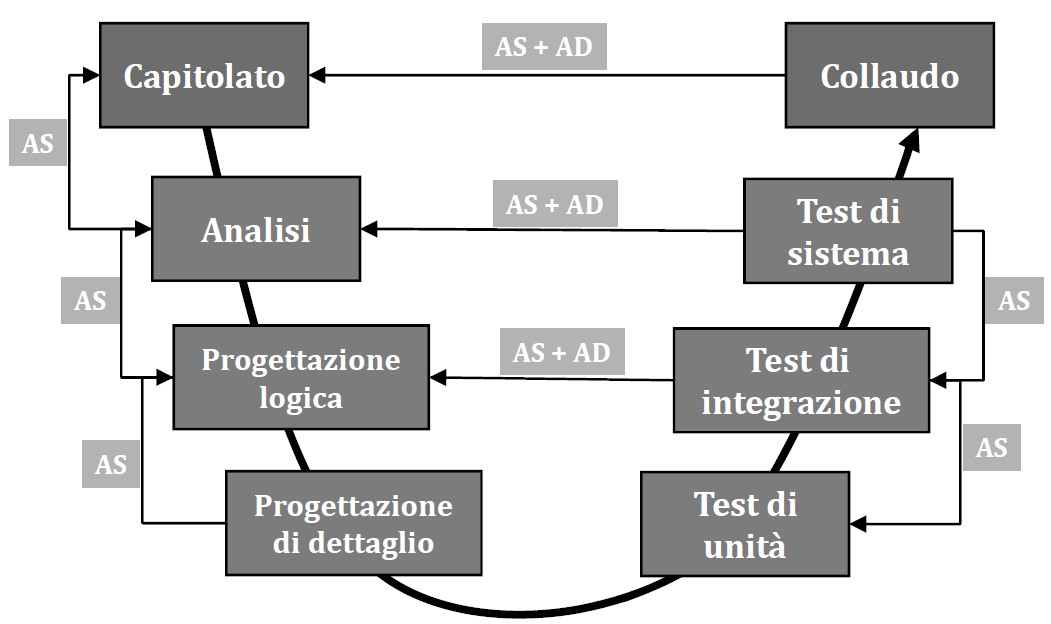
\includegraphics[scale=0.4]{immagini/vmodel2.jpg}
    \end{center}
\end{figure}
\subsection{Analisi statica}
Come è già stato detto, l'analisi statica non richiede software in esecuzione. Inoltre, si applica a ogni prodotto di processo (anche alla documentazione quindi).\newline
Questo tipo di analisi richiede l'utilizzo di una certa tipologia di strumenti che analizzati gli input permettono di restituire ciò che non va, tipicamente dal punto di vista sintattico.
Un'attività che però non può essere svolta da degli strumenti automatici è il controllo di un testo, che deve per forza essere fatto dall'uomo.
Sia la lettura che i controlli automatici possono essere fatti mediante due tipologie di verifica, relativamente complementari: \g{walkthrough} e \g{inspection}.
\subsubsection{Walkthrough}
Il walkthrough è un tipo di verifica che viene fatto nelle prime fasi dello sviluppo. Il suo scopo è quello di verificare la presenza di difetti, errori, criticità tramite un'analisi critica del contenuto dell'oggetto di verifica. Non si assume nulla, si verifica solamente. Alcune strategie possibili per svolgere questo tipo di verifica sono:
\begin{itemize}
    \item Per il codice: leggerlo simulandone l'esecuzione;
    \item Per i documenti: leggerlo attentamente per filo e per segno.
\end{itemize}
Le attività da compiere per un tipo di verifica di tipo walkthrough sono:
\begin{itemize}
    \item Pianificazione di cosa analizzare;
    \item Lettura;
    \item Discussione degli errori riscontrati;
    \item Correzione dei difetti.
\end{itemize}
\subsubsection{Inspection}
L'inspection è un tipo di verifica che viene fatto in fasi dello sviluppo avanzate, e il suo scopo è rilevare la presenza di difetti eseguendo una lettura mirata dell'oggetto di verifica, tramite \textit{error guessing}. Viene svolta non più dal gruppo per intero, come avviene per la verifica di tipo walkthrough, ma dai verificatori.\newline
Le attività da compiere per un tipo di verifica di tipo walkthrough sono:
\begin{itemize}
    \item Pianificazione di cosa analizzare;
    \item Definizione lista di controllo;
    \item Lettura;
    \item Correzione dei difetti.
\end{itemize}
\subsection{Analisi dinamica}
Come è stato già detto, l'analisi dinamica richiede invece il software in esecuzione. L'analisi dinamica si basa sul concetto di test. I test devono essere ripetibili e per questo richiedono che vengano specificati:
\begin{itemize}
    \item Ambiente d'esecuzione: hardware e software, stato iniziale;
    \item Input e output attesi;
    \item Procedure: ciò che deve essere eseguito e controllato.
\end{itemize}
Per automatizzare i test si possono usare degli strumenti:
\begin{itemize}
    \item Driver: componente attiva fittizia che guida l'esecuzione dei test;
    \item Stub: componente passiva fittizia che simula una parte del sistema utile al test ma non l'oggetto sotto test;
    \item Logger: componente che registra gli eventi durante i test, oltre che i risultati.
\end{itemize}
\subsection{Tipi di test}
\begin{figure}[h]
    \begin{center}
        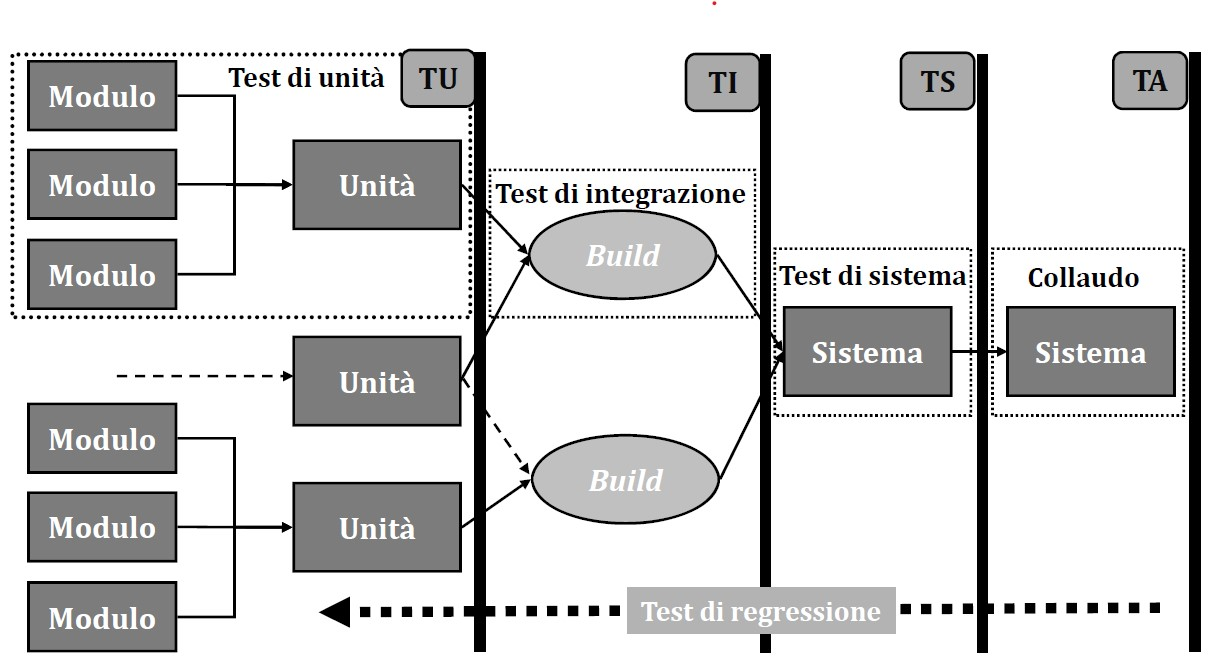
\includegraphics[scale=0.5]{immagini/test.jpg}
    \end{center}
\end{figure}
\subsubsection{Test di unità}
Sono test atti a valutare la correttezza delle \g{unità} software prese singolarmente, per verificare che facciano effettivamente ciò che dichiarano. Ciò comporta che se un'unità è corretta presa da sola, non è detto che presa nell'insieme faccia il suo mestiere.\newline
Le unità sono tante in un \g{prodotto software}, di conseguenza i test di unità sono pure tanti. Devono possibilmente essere eseguiti in parallelo e mediante un automazione.
\subsubsection{Test di regressione}
I test di regressione sono test che servono a verificare che una nuova funzionalità non pregiudichi il funzionamento del sistema già testato precedentemente. Per effettuare questo tipo di test è come minimo necessario rieseguire i test già presenti e, se serve, implementarne di nuovi.
\subsubsection{Test di integrazione}
I test di integrazione sono test in cui si verifica il funzionamento di unità che necessitano di collaborare per raggiungere un risultato. Servono a verificare la corretta integrazione fra le parti. Vanno fatte man mano, con in mente l'approccio del modello incrementale.\newline
Questo tipo di test verifica:
\begin{itemize}
    \item Errori nell'integrazione fra le componenti;
    \item Interfacce errate o cambiamenti nei requisiti;
    \item Componenti con comportamento inadatto.
\end{itemize}
\subsubsection{Test di sistema e collaudo}
I test di sistema, anche conosciuti come collaudo, sono i test che si fanno internamente per per accertare la corretta soddisfazione di tutti i requisiti dell'analisi dei requisiti. Si chiama collaudo quando sono svolti in presenza del committente.
\end{document}